
\section{The Interactions of Electric Charges\footnote{%
Adapted from A. Arons, \underbar{A Guide to Introductory Physics Teaching},
Wiley \& Sons, 1990; and R. Chabay and B. Sherwood, \underbar{Electric
\& Magnetic Interactions}, Wiley \& Sons, 1995.
}}

Name \rule{2.0in}{0.1pt}\hfill{}Section \rule{1.0in}{0.1pt}\hfill{}Date
\rule{1.0in}{0.1pt}

\textbf{Objectives}

\begin{itemize}
\item Note the number of different kinds of charge
\item Characterize the interactions between like and unlike charges
\item Discover the nature of electrical force
\end{itemize}
\textbf{Introduction}

You probably already know this, but electric force between charge
objects is proportional to the amount of charge on each of the objects,
acts along a line between the objects, and decreases rapidly as the
distance between the two objects increases. In the following activities,
you will find out if invisible tape exhibits these properties, and
thus whether such tape becomes electrically charged and therefore
useful in the study of electrical interactions. Use strips of tape
around 20 cm long. Shorter pieces are too inflexible; longer ones
too difficult to handle. Fold one end of each strip to make a non-stick
handle and stick a paper clip on this handle.

Note: The real world is messy. Straight-forward experimental manipulations
and accurate measurements are not always easy to come by. Try to keep
your frustration level down. Rough observations are good enough for
this lab.

\textbf{Apparatus}

\begin{itemize}
\item Invisible ({}``Scotch'') tape
\item Paper clips (2)
\end{itemize}
\textbf{Investigation 1: Your Hand and a U Tape}

\textbf{Preparing a U Tape:}

\begin{enumerate}
\item Stick a strip of tape, sticky-side down, onto the table top and smooth
it down with your thumb or fingers. This base tape provides a standard
work surface and thus ensures consistent results.
\item Stick a second strip of tape, sticky-side down, on top of the base
tape and smooth it down well with thumb or fingertips. Write the letter
U (for Upper) on the handle of this strip.
\item Holding the handle and with a very quick motion, pull the U tape up
and off the base tape, which should remain stuck to the table.
\end{enumerate}
\textbf{Activity:}

\begin{enumerate}
\item Hang the U tape vertically from the edge of the table, handle down.
\item Briefly describe what happens when you slowly bring your hand near
the hanging tape.\vspace{15mm}

\item Is the behavior different when you approach the other side of the
tape?\vspace{15mm}

\end{enumerate}
\textbf{Note:} Tape should react to the presence of your hand. If
not, repeat the U tape preparation.

\textbf{Prediction:} How would you expect two U tapes to interact:
repel each other, attract each other, or not affect each other? Briefly
explain your reasoning.
\vspace{1in}

\textbf{Investigation 2: Two U Tapes}

\textbf{Activity 1:}

\begin{enumerate}
\item Prepare a second U tape, remembering to mark U on its handle.
\item Doing your best to keep your hand out of the way (recall that your
hand attracts the tape--perhaps hold the second strip horizontally
in two hands), bring the second U tape near the hanging first one.
Describe what happens.\vspace{15mm}

\item Hand the second U tape beside the first.
\end{enumerate}
\textbf{Activity 2:}

\begin{enumerate}
\item Suspend a U tape from a piece of thread or hair.
\item Approach the suspended tape from various directions with the other
U tape. Do the tapes repel along or at an angle to the line between
the objects?
\end{enumerate}
\vspace{0.3cm}
{\centering 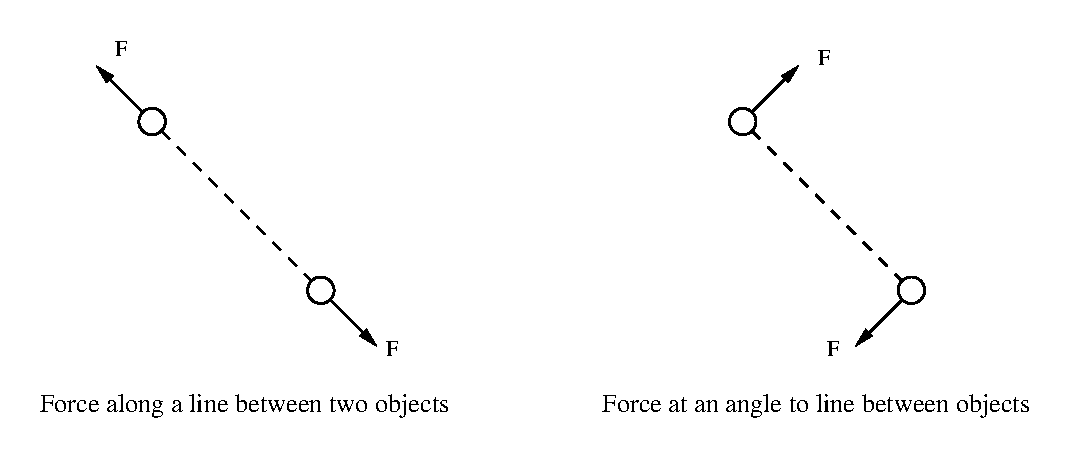
\includegraphics{int_elec_charges_fig_1.eps} \par}
\vspace{0.3cm}

\vspace{15mm}
\textbf{Note:} You may have noticed that if you handle a U tape too
much, it loses its interaction strength. Remember to reactivate the
strips regularly.

\textbf{Activity 3:}

\begin{enumerate}
\item Note that when you move one U tape slowly toward a hanging U tape,
there is a distance at which repulsion is first detectable.
\item Note what happens as you repeatedly halve the distance between the
strips.\vspace{15mm}

\item Graph--very roughly--the deflection of the hanging tape as a function
of the distance between tapes. Note that this deflection from an original
vertical position is a measure of the strength of the interaction.
\end{enumerate}
\vspace{0.3cm}
{\centering \includegraphics{int_elec_charges_fig_2.eps} \par}
\vspace{0.3cm}

\textbf{Activity 4:}

\begin{enumerate}
\item Hold the bottom of a hanging, active U tape and slowly rub your thumb
or fingers back and forth along its slick side.
\item Describe the changes in how this U tape interacts with your hand.
Also, with another U tape.\vspace{15mm}

\item Reactivate two U tapes. Hang one from the table and note how strongly
the other one repels it.\vspace{15mm}

\item Run a finger along the length of the hanging tape's slick side, but
touch only a portion of its width (not the full side). Be sure to
leave a continuous vertical section untouched. 
\item Do the two tapes now exhibit a weaker or stronger repulsion, or no
repulsion at all?\vspace{15mm}

\item Try to explain what has been going on in this activity.\vspace{15mm}

\end{enumerate}
\textbf{Questions:}

\begin{enumerate}
\item Are U tapes electrically charged?\vspace{10mm}

\item Do U tapes have like or unlike electric charge?\vspace{10mm}

\end{enumerate}
\textbf{Investigation 3: A U and an L Tape}

\textbf{Challenge:} How would you prepare a tape that might have an
electric charge unlike the charge on a U tape?

\textbf{Preparing an L Tape:}

\begin{enumerate}
\item Stick a strip of tape, sticky-side down, on top of the base tape and
smooth it down well with thumb or fingertips. Write the letter L (for
Lower) on the handle of this strip.
\item Stick a second strip of tape, sticky-side down, on top of the L tape
and smooth it down well with thumb or fingertips. Write the letter
U (for Upper) on the handle of this strip.
\item Lifting the handle of the L tape, slowly pull it along with the U
tape up and off the base tape, which should remain stuck to the table.
\item Hang the double layer of tape vertically from the edge of the table,
handles down. Check that there is no interaction between it and your
hand. If there is, do what you need to so the interaction no longer
occurs.
\item While holding down the handle of the L tape, quickly life off the
U tape, then hang it vertically from the edge of the table, not too
close to the L tape.
\end{enumerate}
\textbf{Prediction:} Will the L tape attract, repel, or not interact
with the U tape if the two are brought within proximity of one another?
\vspace{1in}

\textbf{Activity 1:}

\begin{enumerate}
\item With your hand, check that both the U tape and the L tape are active.
How can you tell?\vspace{15mm}

\item What interaction do you observe between an L tape and a U tape?\vspace{15mm}

\end{enumerate}
\textbf{Prediction:} Will an L tape attract, repel, or not interact
with another L tape if the two are brought within proximity of one
another?
\vspace{15mm}

\textbf{Activity 2:}

\begin{enumerate}
\item Make another pair of L and U tapes.
\item Be sure that all four tapes are active.
\item What interaction do you observe between two L tapes?\vspace{15mm}

\item Summarize the interactions you have observed between U and L tapes:
\end{enumerate}
\begin{quote}
L-U:

U-U:

L-L:
\end{quote}
~~~~5.~State a rule for the pattern of interactions between like
and unlike charges:
\vspace{20mm}

\textbf{Activity 3:}

\begin{enumerate}
\item Note that when you move an active L tape slowly toward a hanging U
tape, there is a distance at which attraction is first detectable.
\item Note what happens as you repeatedly halve the distance between the
strips.\vspace{15mm}

\item Graph--very roughly--the deflection of the hanging tape as a function
of the distance between tapes. Note that this deflection from an original
vertical position is a measure of the strength of the interaction.
\end{enumerate}
\vspace{0.3cm}
{\centering \includegraphics{int_elec_charges_fig_3.eps} \par}
\vspace{0.3cm}

\textbf{Questions:}

\begin{enumerate}
\item Why is this task more difficult now than it was with two U tapes?\vspace{15mm}

\item Do the forces between U and L tapes lie along or at an angle to the
line between the tapes?
\end{enumerate}
\begin{quotation}
Force by U tape on L tape:
\vspace{10mm}

Force by L tape on U tape:\vspace{10mm}

\end{quotation}
\textbf{Summary:} In the table below, state very briefly what you
observed.

\vspace{0.3cm}
{\centering \begin{tabular}{|l|l|}
\hline 
~~~~~~~~~~~~~~~~~~~~~~~~~~~~~~~~\textbf{Property}&
\textbf{Experimental Observation of U and L Tapes}\\
\hline
\hline 
There are two kinds of charges;&
U-U:\\
like charges repel;&
L-L:\\
unlike charges attract.&
U-L:\\
\hline 
Electric force is proportional to amount of charge.&
U tape and partially neutralized U tape:\\
&
\\
\hline 
Electric force acts along a line between charges.&
U-U:\\
&
U-L:\\
\hline 
The strength of interaction decreases&
U-U:\\
rapidly as distance between the charges increases.&
U-L:\\
\hline
\end{tabular}\par}
\vspace{0.3cm}

\textbf{Activity 4:}

\begin{enumerate}
\item Quickly lift off the base tape.
\item Is it U-like or L-like? How can you tell?\vspace{15mm}

\end{enumerate}
\textbf{Questions:}

\begin{enumerate}
\item How does all of this happen: How do the tapes become charged? Why
are both U and L tapes attracted to your hand? Why does rubbing the
slick side of a tape with your finger appear to neutralize the tape?\vspace{20mm}

\item What do you think charges are?\vspace{15mm}
\end{enumerate}

